% !Mode:: "TeX:UTF-8"
%!TEX program  = xelatex

\documentclass{cumcmthesis}
%\documentclass[withoutpreface,bwprint]{cumcmthesis} %去掉封面与编号页

\usepackage{url}
\usepackage{tikz}
\usepackage{xcolor}
\usepackage{graphicx} % 图片插入需要的宏包
\usepackage{float}
\usepackage{subcaption}
\usetikzlibrary{patterns}
\title{全国大学生数学建模竞赛编写的 \LaTeX{} 模板}
\tihao{A}
\baominghao{4321}
\schoolname{XX大学}
\membera{小米}
\memberb{向左}
\memberc{哈哈}
\supervisor{老师}
\yearinput{2017}
\monthinput{08}
\dayinput{22}

\begin{document}

 \maketitle
 \begin{abstract}
cumcmthesis 是为全国大学生数学建模竞赛编写的\LaTeX{}模板, 旨在让大家专注于 论文的内容写作, 而不用花费过多精力在格式的定制和调整上. 本手册是相应的参考, 其 中提供了一些环境和命令可以让模板的使用更为方便. 同时需要注意, 使用者需要有一 定的 \LaTeX{} 的使用经验, 至少要会使用常用宏包的一些功能, 比如参考文献,数学公式,图片使用,列表环境等等. 例子文件参看 example.pdf.

另外, 欢迎大家购买我们是视频教程,点击\href{https://item.taobao.com/item.htm?spm=a1z10.1-c.w4004-3473795048.4.ThFQCG&id=43823508044}{\fbox{这里}}。

欢迎大家到QQ群里沟通交流:91940767.

\uwave{关注我们的微信公众号}:

\centerline{
\includegraphics[width=5cm]{gongzhonghao}}

\keywords{折叠桌\quad  曲线拟合\quad   非线性优化模型\quad  受力分析}
\end{abstract}

%目录
\tableofcontents

















\clearpage
\section{问题重述}
\subsection{问题背景}
近年来,随着社会经济的发展和生活方式的改变,慢性病在全球范围内显著上升,成为危害人类健康的重要公共卫生问题。慢性病的发展与个体的生活方式紧密相关。生活方式因素,如饮食习惯、体育锻炼、吸烟、饮酒等,被认为在慢性病的发生和发展中扮演着重要角色。不同的饮食结构、身体活动水平和生活习惯可能对慢性病的风险产生显著影响。为了更好地理解这种关联,必须进行深入研究,以便制定更精确的预防和干预策略。

\subsection{问题的提出}


根据所给表格数据,统计居民的各类饮食习惯,并与附件A3中所给出的中国居民膳食指南八条准则进行对比,从而对居民饮食习惯的合理性进行分析。


\section{模型的假设}

\begin{itemize}
\item 我们一个月按照30天/4周来计算
\end{itemize}

\section{符号说明}
\begin{table}[h!]
  \centering
  \small
  \begin{tabular}{p{60pt}<{\centering}|p{60pt}<{\centering}p{180pt}<{\raggedright}}
   \hline
    序号 & 符号 & 符号说明 \\
   \hline
    1 & $\mathbf{D}$ & 微分算子 \\
    \hline
  \end{tabular}
  %\caption{符号与说明}
  \label{symbol}
\end{table}
\section{问题分析}

\subsection{问题一分析}
题目要求建立模型描述折叠桌的动态变化图,由于在折叠时用力大小的不同,我们不能描述在某一时刻折叠桌的具体形态,但我们可以用每根木条的角度变化来描述折叠桌的动态变化。首先,我们知道折叠桌前后左右对称,我们可以运用几何知识求出四分之一木条的角度变化。最后,根据初始时刻和最终形态两种状态求出桌腿木条开槽的长度。


\section{问题一求解}
本题数据为问卷数据,对于问卷数据的处理包括数据资料的整理和数据资料的分析。

我们首先对异常问卷数据进行处理。对于一些可能由于填写错误引起的问卷异常,我们选择保留该项数据。例如问题D1-D3中一周吃早/中/晚餐和不吃早/中/晚餐天数加起来超过7天,这与事实不符,我们选择调整其不吃的天数使其符合事实。在问题D4-D30中,对于填写了b选项食用频率而a选项选择不食用该项食物的问卷,我们选择将其a选项是否食用更正为食用。对于一些无效问卷未完成的问卷、随意填答等问卷,我们可以将其视为无效问卷,进行删除该问卷数据处理。在问题D31-D37中,由于数据量较大我们认为数据符合正太分布,选择用$3\sigma$原则对离群问卷数据进行删除处理,对于问卷中的缺失数据,我们选择用该项数据的平均值进行填充。

接下来我们将数据处理为各食物每月的食用频率以及食用量,我们就可以得到各食物平均食用频率、食用人数占比以及平均每月食用量。结果见表\ref{1}:
\begin{table}[!ht]
\centering
\caption{饮食习惯数据}
\label{1}\resizebox{\textwidth}{!}{
\begin{tabular}{ccccc}
\hline
食物编号 & 食物类型             & 平均食用频率(次/月) & 食用人数占比(\%)  & 平均每天食用量(g)  \\ \hline
D4   & 大米               & 60.8219755  & 99.2215416  & 106.978332  \\
D5   & 小麦面粉             & 10.60548749 & 82.36345074 & 96.1044876  \\
D6   & 杂粮(小米/高粱/玉米/红豆等) & 4.947026544 & 77.71822358 & 86.82923211 \\
D7   & 薯类(红薯/山药芋头/土豆等)  & 4.809290454 & 84.44359367 & 56.49160422 \\
D8   & 油炸面食(油条/油饼等)     & 1.449489535 & 34.4691169  & 73.82573823 \\
D9   & 猪肉               & 41.99226646 & 98.07299643 & 80.25228733 \\
D10  & 牛、羊肉             & 3.287149056 & 68.89994895 & 87.11473284 \\
D11  & 禽肉               & 7.458154671 & 93.72128637 & 110.625431  \\
D12  & 内脏类              & 2.157771822 & 55.57682491 & 67.08697799 \\
D13  & 水产品              & 13.21064319 & 94.55079122 & 117.222545  \\
D14  & 鲜奶               & 7.251237876 & 53.67534456 & 228.2813746 \\
D15  & 奶粉               & 1.089497192 & 8.843797856 & 25.09025102 \\
D16  & 酸奶               & 5.205985197 & 49.56610516 & 198.5220289 \\
D17  & 蛋类               & 12.5110388  & 95.67381317 & 67.96986837 \\
D18  & 豆腐               & 7.233958652 & 92.02399183 & 96.56758454 \\
D19  & 豆腐丝/千张/豆腐干       & 2.487059724 & 48.45584482 & 76.7511263  \\
D20  & 豆浆               & 7.50553854  & 74.24706483 & 194.3994906 \\
D21  & 干豆类(黄豆/黑豆/青豆)    & 3.493797856 & 64.98213374 & 70.35392331 \\
D22  & 新鲜蔬菜             & 55.61294028 & 98.67279224 & 156.1687009 \\
D23  & 海带、紫菜等海草类        & 3.693300153 & 77.75650842 & 62.62388263 \\
D24  & 咸菜               & 3.685528331 & 62.697805   & 43.25351803 \\
D25  & 泡菜               & 1.210056151 & 25.45941807 & 41.60947058 \\
D26  & 酸菜               & 1.875816743 & 46.60541092 & 50.44473056 \\
D27  & 糕点               & 5.449042879 & 72.91985707 & 89.21277463 \\
D28  & 新鲜水果             & 26.70179939 & 97.67738642 & 167.4840718 \\
D29  & 果汁饮料             & 5.13140633  & 56.68708525 & 327.5441622 \\
D30  & 其他饮料             & 5.20086779  & 47.52424706 & 376.3493154 \\ \hline
\end{tabular}}
\end{table}

从表格中可以看出,居民以大米为主食,食用人数占比达到99.2\%,每天食用的膳食基本包括了谷薯类、蔬菜水果、禽畜鱼蛋和豆类食物。摄入食物种类也能够保证一天12种以上。居民对奶类食用频率不达标,平均食用频率13.5次/月,平均每天食用量为451.9g,由此可见应当适量提高奶制品使用频率。居民平均每天摄入蔬菜的量仅有156.1g,新鲜水果摄入量也仅达到161.5g,略低于每天应摄入量,居民应提高新鲜蔬菜水果的摄入量。居民每周摄入水产品和鸡蛋的频率和摄入量达标,鱼禽、蛋类和禽肉的平均摄入量达到295.9g,高于正常摄入水平,应减少鱼肉蛋类的摄入量。

平衡居民膳食的八条准则中提出要培养清淡的饮食习惯,由表\ref{1}可知,居民们对高盐食品,如咸菜、泡菜、酸菜等的每月食用量平均为12.9两,食用频率和食用人数占比则以咸菜居多,可达62.7\%。油炸面食的食用人数占比达到了34.5\%,平均每月食用量将近2两。高糖类食品的摄入更是难以控制,糕点类、新鲜水果、各种饮料的食用人数占比和食用量都是一个不小的数字。居民们不合理的饮食习惯体现在平日不清淡的饮食中。

各种饮料的每月摄入量可达7杯,饮料的过多摄入会对人体健康产生极大的不良影响,包括体重增加、消耗维生素等矿物质、增加患肾脏疾病的风险,甚至还可能导致骨质疏松症等。因此,居民在饮食习惯上应当有节制,尽量减少对含糖饮料和果汁类饮料的摄入,以免对自身的健康造成不良的影响。

 准则中要求成人每天摄入的油量为25~30g,由附件中所给数据进行转换,由于问卷中的食用油量调查单位为斤/月,换算可得一个月的食用量应该置于1.5~1.8斤之间才算符合标准。通过excel表格进行筛选可得出符合标准的居民数量仅有66个,占全部调查人数的0.86\%。由图\ref{t11}可知,绝大部分居民对于少油这一健康的膳食准则并未很好的执行,仍然有过多摄入烹调油这一不合理的饮食习惯。

 健康的饮食习惯应当尽量减少调味料的摄入,由所给数据可得,几乎所有的居民都食用调味料。平衡居民膳食的准则中提出了居民们每天的食用盐用量应该少于5g,附件所给数据为每月平均用量,经过换算可得一个月的食用量应该小于3两才是健康的用量。同样通过excel表格进行筛选,可以得出符合标准的居民数量只有604个,占全部调查数量的7.8\%。由此可知,绝大多数居民仍然无法控制使用食盐的用量,仍然存在着过多摄入食盐这一饮食习惯方面的问题。健康的饮食习惯应当尽量减少调味料的摄入,由所给数据可得,几乎所有的居民都食用调味料。平衡居民膳食的准则中提出了居民们每天的食用盐用量应该少于5g,附件所给数据为每月平均用量,经过换算可得一个月的食用量应该小于3两才是健康的用量。同样通过excel表格进行筛选,可以得出符合标准的居民数量只有604个,占全部调查数量的7.8\%。由此可知,绝大多数居民仍然无法控制使用食盐的用量,仍然存在着过多摄入食盐这一饮食习惯方面的问题。
\begin{figure}[H]
  \centering

  \begin{subfigure}[b]{0.45\textwidth}
    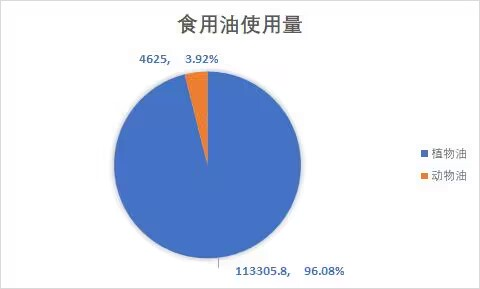
\includegraphics[width=\textwidth]{figures/QQ图片20230813183040.jpg}
    \caption{食用油使用量}
    \label{t11}
  \end{subfigure}
  \hfill
  \begin{subfigure}[b]{0.45\textwidth}
    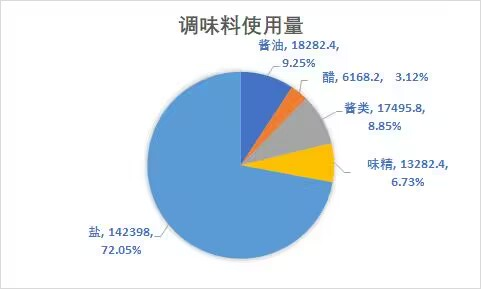
\includegraphics[width=\textwidth]{figures/QQ图片20230813170545.jpg}
    \caption{调味料使用量}
    \label{t12}
  \end{subfigure}
  \caption{食用油及调味料食用量}
\end{figure}
% 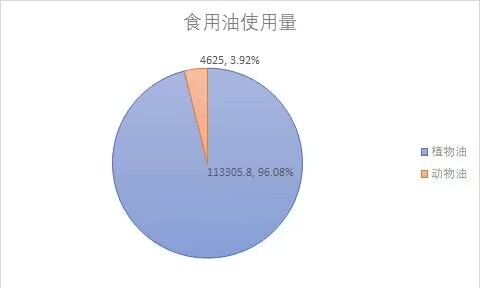
\includegraphics[width=0.4\textwidth]{figures/QQ图片20230813170116.jpg}
% 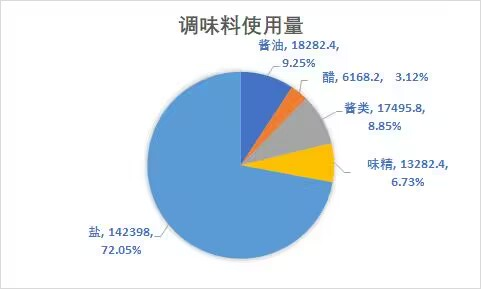
\includegraphics[width=0.4\textwidth]{figures/QQ图片20230813170545.jpg}

% \end{figure}



无论男女老少,酒精的过多摄入都是不利于健康的,由图  数据可得,仍然有很多居民饮酒,且对各类酒的平均每次饮用量也普遍较多不符合膳食准则所要求的酒精量,一部分居民仍然存在不适量饮酒的健康问题。
\clearpage
\section{问题二模型建立和求解}
要分析居民的生活习惯和饮食习惯与年龄、性别、婚姻状况、文化程度、职业等因素的相关性,我们采取$\text{Kendall-}\tau$相关系数来判定。
\subsection{$\text{Kendall}$相关性分析}
对于定类变量我们计算其$\text{Kendall-}\tau$系数度量相关性强弱,$\text{Kendall-}\tau$通过计算两个变量的所有可能观测对之间的一致对和不一致对的数量来计算,如式\ref{s1}所示:
\begin{eqnarray}
\text{Kendall-}\tau=\frac{\sum_{i<k}\sum_{j<l}n_{ij}n_{kl}-\sum_{i<k}\sum_{j>l}n_{ij}n_{kl}}{\sqrt{(\frac{n_{++}(n_{++}-1)}{2}-\frac{\sum_in_{i+}(n_{i+}-1)}{2})(\frac{n_{++}(n_{++}-1)}{2}-\frac{\sum_jn_{+j}(n_{+j}-1)}{2}})}\label{s1}
\end{eqnarray}
其中,$n_{i+}$表示第$i$行观测值数,$n_{+j}$表示第$j$列观测值数,$n_{ij}$表示第$i$行第$j$列的观测值,$n_{++}$表示观测值总数。

我们通过计算得到年龄、性别、婚姻状况、文化程度、职业等因素与生活习惯与饮食习惯的$\text{Kendall-}\tau$系数,结果见图\ref{2}:
\begin{figure}[H]
\centering
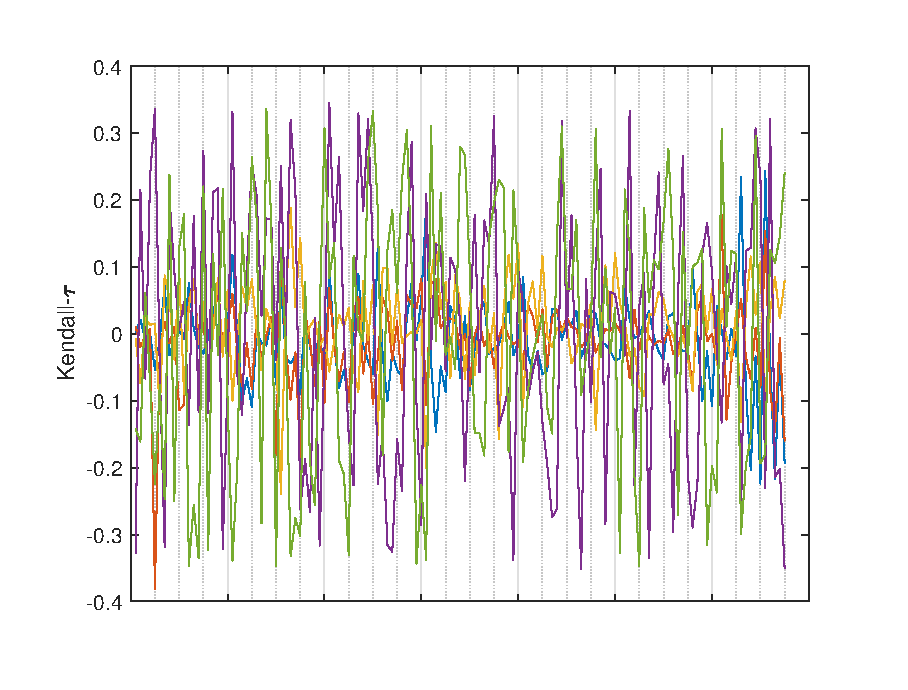
\includegraphics{figures/A2.eps}
\caption{$\text{Kendall-}\tau$系数}\label{2}
\end{figure}

以性别和饮食习惯为例,我们将$\text{Kendall-}\tau$系数从高到低排序并绘制如图\ref{3}所示。我们发现${Kendall-}\tau$相关系数绝对值均不超过0.3,我们认为不存在显著相关性。
\begin{figure}[H]
\centering
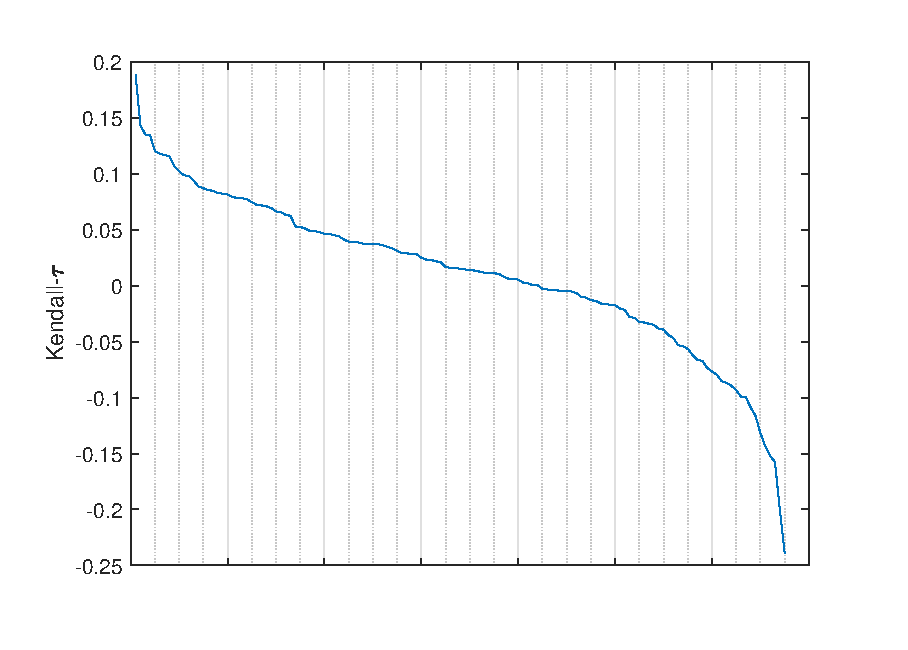
\includegraphics{figures/A1.eps}
\caption{性别与饮食习惯的$\text{Kendall-}\tau$系数}\label{3}
\end{figure}
\section{问题三模型建立与求解}
















\section{绘制普通三线表格}
表格应具有三线表格式,因此常用 booktabs宏包,其标准格式如表~\ref{tab001}~所示。
\begin{table}[!htbp]
\caption{标准三线表格}\label{tab001} \centering
\begin{tabular}{ccccc}
\toprule[1.5pt]
$D$(in) & $P_u$(lbs) & $u_u$(in) & $\beta$ & $G_f$(psi.in)\\
\midrule[1pt]
 5 & 269.8 & 0.000674 & 1.79 & 0.04089\\
10 & 421.0 & 0.001035 & 3.59 & 0.04089\\
20 & 640.2 & 0.001565 & 7.18 & 0.04089\\
\bottomrule[1.5pt]
\end{tabular}
\end{table}

其绘制表格的代码及其说明如下。
\begin{tcode}
\begin{table}[!htbp]
\caption[标签名]{中文标题}
\begin{tabular}{cc...c}
\toprule[1.5pt]
表头第1个格   & 表头第2个格   & ... & 表头第n个格  \\
\midrule[1pt]
表中数据(1,1) & 表中数据(1,2) & ... & 表中数据(1,n)\\
表中数据(2,1) & 表中数据(2,2) & ... & 表中数据(2,n)\\
...................................................\\
表中数据(m,1) & 表中数据(m,2) & ... & 表中数据(m,n)\\
\bottomrule[1.5pt]
\end{tabular}
\end{table}
\end{tcode}

\bigskip
table环境是一个将表格嵌入文本的浮动环境。
tabular环境的必选参数由每列对应一个格式字符所组成:c表示居中,l表示左对齐,r表示右对齐,其总
个数应与表的列数相同。此外,\verb|@{文本}|可以出现在任意两个上述的列格式之间,其中的文本将被插入每一行
的同一位置。表格的各行以\verb|\\|分隔,同一行的各列则以\&分隔。
\verb|\toprule|、\verb|\midrule|和\verb|\bottomrule|三个命令是由booktabs宏包提供的,其
中\verb|\toprule|和\verb|\bottomrule|分别用来绘制表格的第一条(表格最顶部)和第三条(表格最底部)水平线,
\verb|\midrule|用来绘制第二条(表头之下)水平线,且第一条和第三条水平线的线宽为1.5pt,第二条水平线的线宽为1pt。
引用方法:“如表~\verb|\ref{标签名}|~所示”。


%参考文献
\begin{thebibliography}{9}%宽度9
 \bibitem{bib:one} ....
 \bibitem{bib:two} ....
\end{thebibliography}

\newpage
%附录
\begin{appendices}
\section{排队算法--matlab 源程序}
\begin{lstlisting}[language=matlab]
kk=2;[mdd,ndd]=size(dd);
while ~isempty(V)
[tmpd,j]=min(W(i,V));tmpj=V(j);
for k=2:ndd
[tmp1,jj]=min(dd(1,k)+W(dd(2,k),V));
tmp2=V(jj);tt(k-1,:)=[tmp1,tmp2,jj];
end
tmp=[tmpd,tmpj,j;tt];[tmp3,tmp4]=min(tmp(:,1));
if tmp3==tmpd, ss(1:2,kk)=[i;tmp(tmp4,2)];
else,tmp5=find(ss(:,tmp4)~=0);tmp6=length(tmp5);
if dd(2,tmp4)==ss(tmp6,tmp4)
ss(1:tmp6+1,kk)=[ss(tmp5,tmp4);tmp(tmp4,2)];
else, ss(1:3,kk)=[i;dd(2,tmp4);tmp(tmp4,2)];
end;end
dd=[dd,[tmp3;tmp(tmp4,2)]];V(tmp(tmp4,3))=[];
[mdd,ndd]=size(dd);kk=kk+1;
end; S=ss; D=dd(1,:);
 \end{lstlisting}
 \section{规划解决程序--lingo源代码}
\begin{lstlisting}[language=c]
kk=2;
[mdd,ndd]=size(dd);
while ~isempty(V)
    [tmpd,j]=min(W(i,V));tmpj=V(j);
for k=2:ndd
    [tmp1,jj]=min(dd(1,k)+W(dd(2,k),V));
    tmp2=V(jj);tt(k-1,:)=[tmp1,tmp2,jj];
end
    tmp=[tmpd,tmpj,j;tt];[tmp3,tmp4]=min(tmp(:,1));
if tmp3==tmpd, ss(1:2,kk)=[i;tmp(tmp4,2)];
else,tmp5=find(ss(:,tmp4)~=0);tmp6=length(tmp5);
if dd(2,tmp4)==ss(tmp6,tmp4)
    ss(1:tmp6+1,kk)=[ss(tmp5,tmp4);tmp(tmp4,2)];
else, ss(1:3,kk)=[i;dd(2,tmp4);tmp(tmp4,2)];
end;
end
    dd=[dd,[tmp3;tmp(tmp4,2)]];V(tmp(tmp4,3))=[];
    [mdd,ndd]=size(dd);
    kk=kk+1;
end;
S=ss;
D=dd(1,:);
 \end{lstlisting}
\end{appendices}

\end{document} 